\section{Постановка задачи. Обзор предметной области}

Данный раздел содержит обзор предметной области по теме дипломного проекта, аналоги создаваемого программного продукта, анализ их достоинств и недостатков. На основе проведенного анализа и с учетом требований формулируются требования к проектируемому программному средству.


\subsection{Постановка задачи}

Цель настоящего дипломного проекта состоит в разработке компьютерной игры \BinaryWars, представляющая собой продвинутый аналог игры \TicTacToe, которая призвана разнообразить досуг людей, предоставив им возможность сыграть в знакомую классическую игру, но в совершенно новом виде и с новыми возможностями. Также своей целью автор данного дипломного проекта ставит разработку кодовой базы с использованием различных современных техник написания кода для стабильной и быстрой работы программного продукта на широком круге целевых устройств, в том числе для обеспечения дополнения и изменения кода без влияния на другие части проекта, а также возможность использовать полученный код в будущих проектах.

При постановке задачи были сформулированы следующие требования к проектируемому программному средству:
\begin{enumerate}[label=\arabic*, itemindent=\parindent + 2.3ex]
    \item Целевыми платформами являются мобильные устройства под управлением операционных систем Android и iOS.
    \item Наличие помимо классического игрового режима (двухмерное игровое поле три на три клетки) игрового режима с трёхмерным игровым полем.
    \item Возможность игры против компьютерного противника, при этом он должен достаточно быстро обрабатывать свой ход, иметь возможность настройки уровня сложности и работать в рамках различных игровых режимов.
    \item Обязательно наличие кроссплатформенной многопользовательской игры со случайным или определённым оппонентом, при этом для игроков создание или присоединение к игровой сессии должно происходить в максимально простой и удобной манере. Также у игроков должна присутствовать возможность общения в процессе игры посредством внутриигрового чата.
    \item Должен присутствовать внутриигровой магазин с возможностью совершения покупок за реальные деньги.
    \item Следует обеспечить возможность пользователю изменять настройки программного продукта: включать или выключать звуковые эффекты, музыку, графические эффекты, возможность изменения имени игрока и восстановления покупок во внутриигровом магазине и т.п.
    \item Игра должна иметь оригинальный и легко узнаваемый визуальный стиль для привлечения большего числа потребителей.
\end{enumerate}


\subsection{Обзор существующих аналогов}

Для того, чтобы удостовериться в актуальности создаваемого программного продукта для реализации на рынке, был произведён анализ некоторых аналогов данного продукта, представленный ниже.


\subsubsection{Крестики-нолики 2 (BYRIL)}

Крестики-нолики 2 (BYRIL) -- самая популярная версия игры среди всех других версий на операционной системе Android. Игра обладает приятным визуальным стилем (рисунки \ref{Figure:Analysis:BYRILMainMenu} и \ref{Figure:Analysis:BYRILGameplay}) а также присутствует возможность как многопользовательской игры по сети интернет, так и игры против компьютерного противника \cite{BYRIL}.

К минусам приложения можно отнести следующее:
\begin{itemize}
    \item отсутствует игровой режим с трёхмерным игровым полем;
    \item отсутствует версия под операционную систему iOS;
    \item для многопользовательской игры по сети интернет требуется наличие у пользователя сторонних сервисов;
    \item игра не всегда ведёт себя стабильно, что может привести к зависанию и вылету игры.
\end{itemize}

\begin{figure}
    \centering
    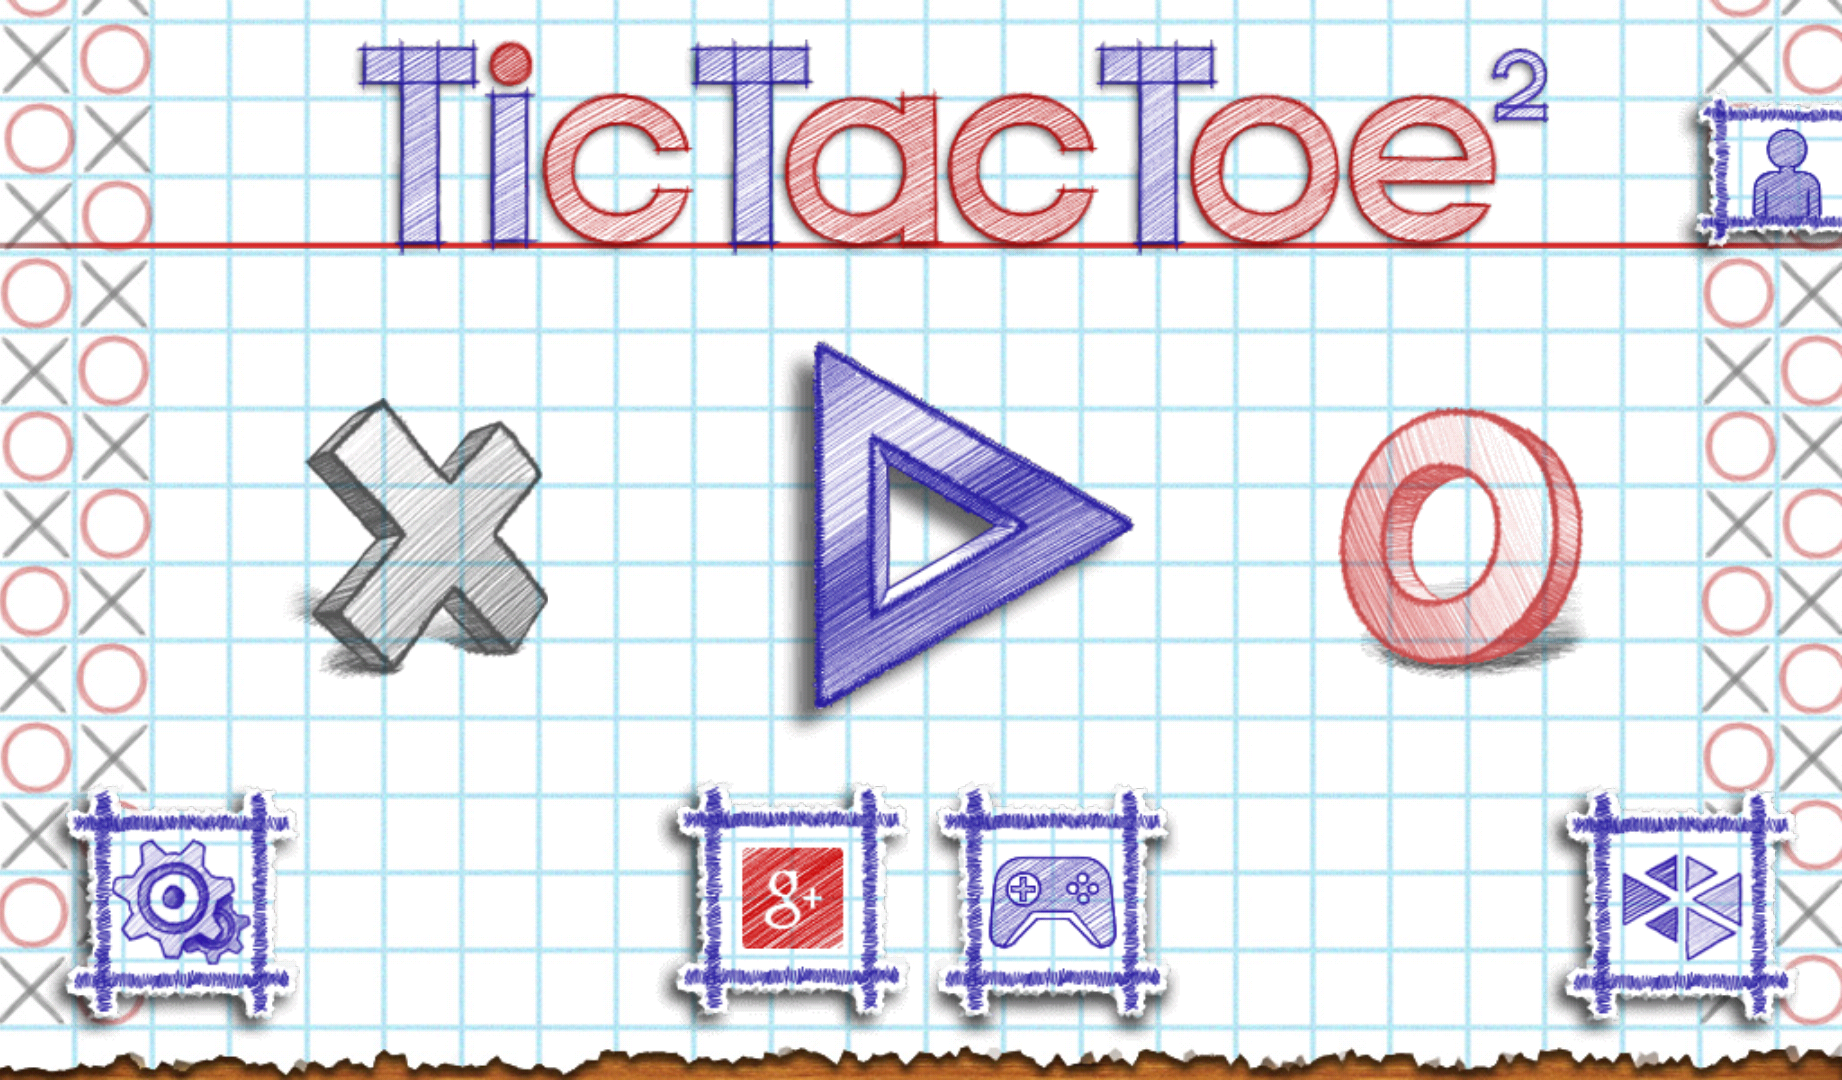
\includegraphics[width=15cm, keepaspectratio]{Analogs/BYRILMainMenu.png}
    \caption{Главное меню игры Крестики-нолики 2 (BYRIL)}
    \label{Figure:Analysis:BYRILMainMenu}
\end{figure}

\begin{figure}
    \centering
    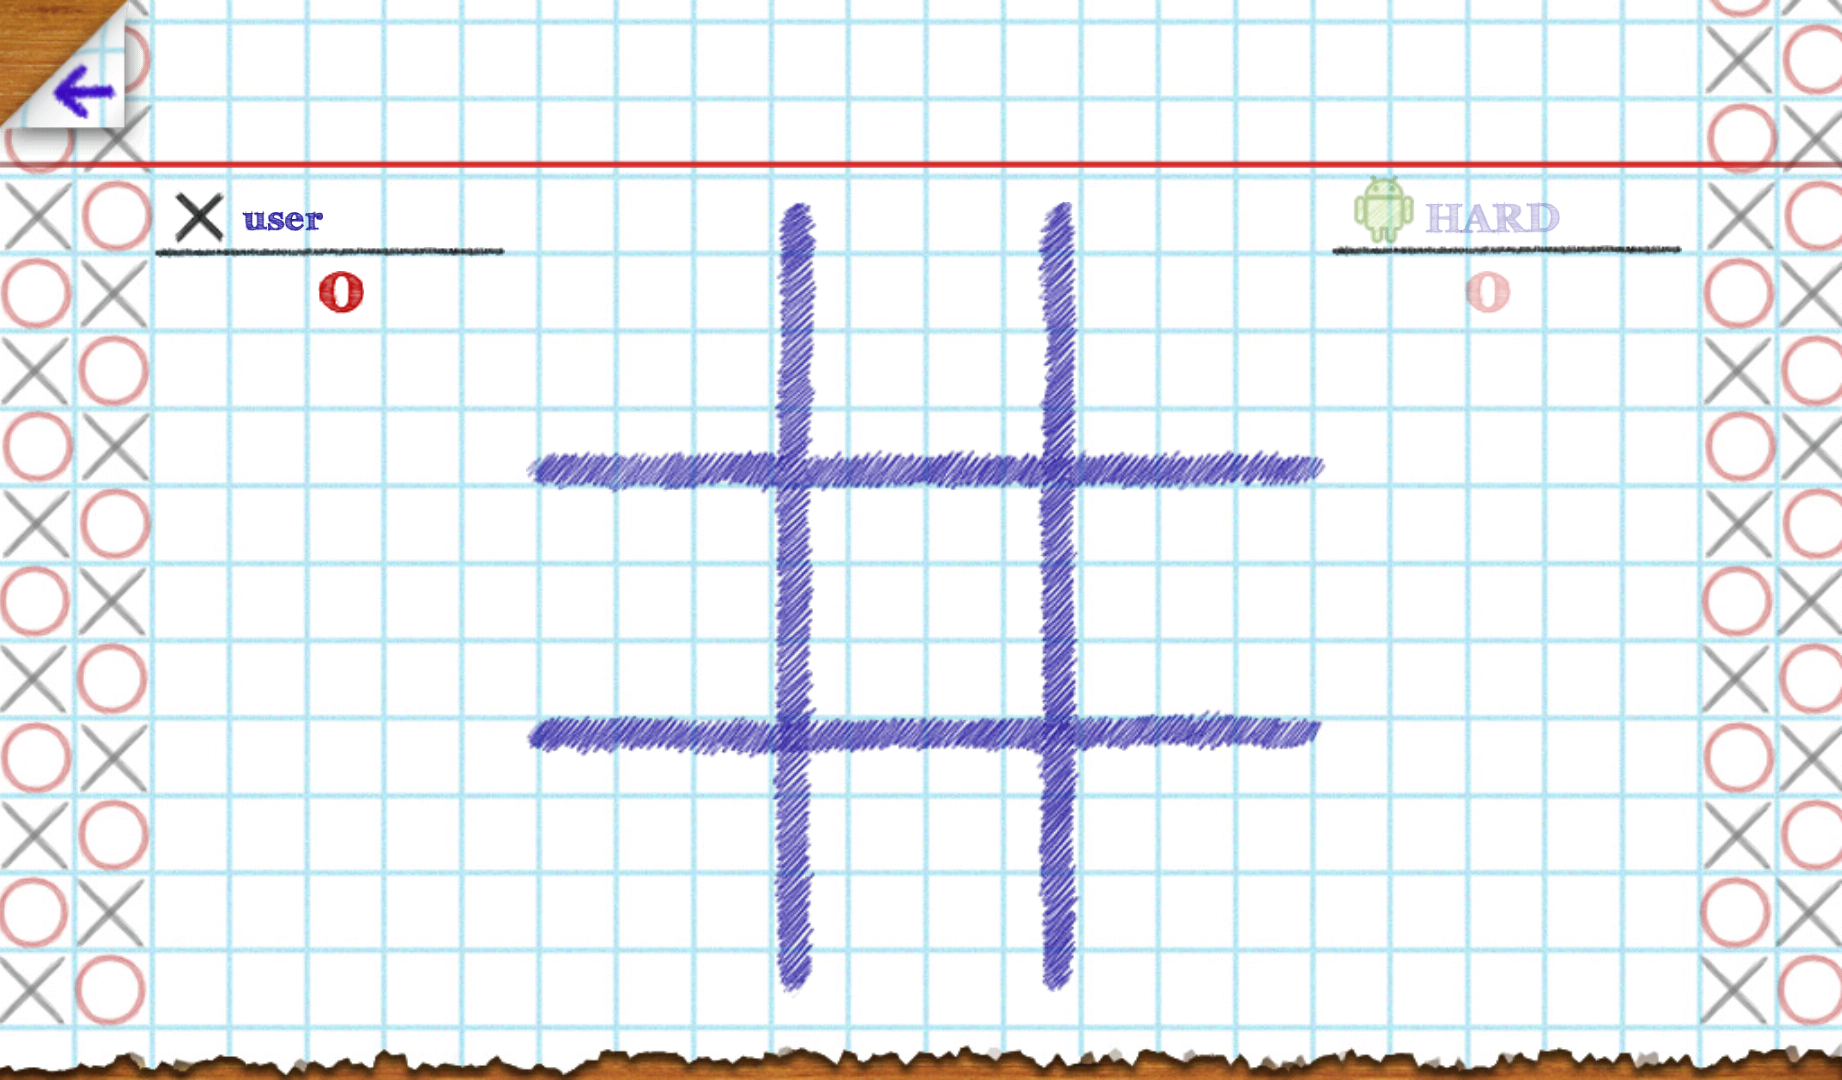
\includegraphics[width=15cm, keepaspectratio]{Analogs/BYRILGameplay.png}
    \caption{Игровой процесс игры Крестики-нолики 2 (BYRIL)}
    \label{Figure:Analysis:BYRILGameplay}
\end{figure}


\subsubsection{Tic Tac Toe Pro (aimlesscreativity)}

Tic Tac Toe Pro (aimlesscreativity) -- версия игры, игровое поле в которой полностью выполнено с помощью трёхмерной графики. Из достоинств можно отметить небольшие системные требования к устройству и высокое энергосбережение, также присутствует игровой режим на трёхмерном игровом поле \cite{Aimlesscreativity}.

К минусам приложения можно отнести следующее:
\begin{itemize}
    \item у игры отсутствует свой визуальный стиль и не самое удобное управление (рисунок \ref{Figure:Analysis:AimlesscreativityGameplay});
    \item отсутствует возможность многопользовательской игры;
    \item отсутствует версия под операционную систему iOS;
    \item разработчик не выпускал обновлений игры с 2013 года.
\end{itemize}

\begin{figure}
\centering
    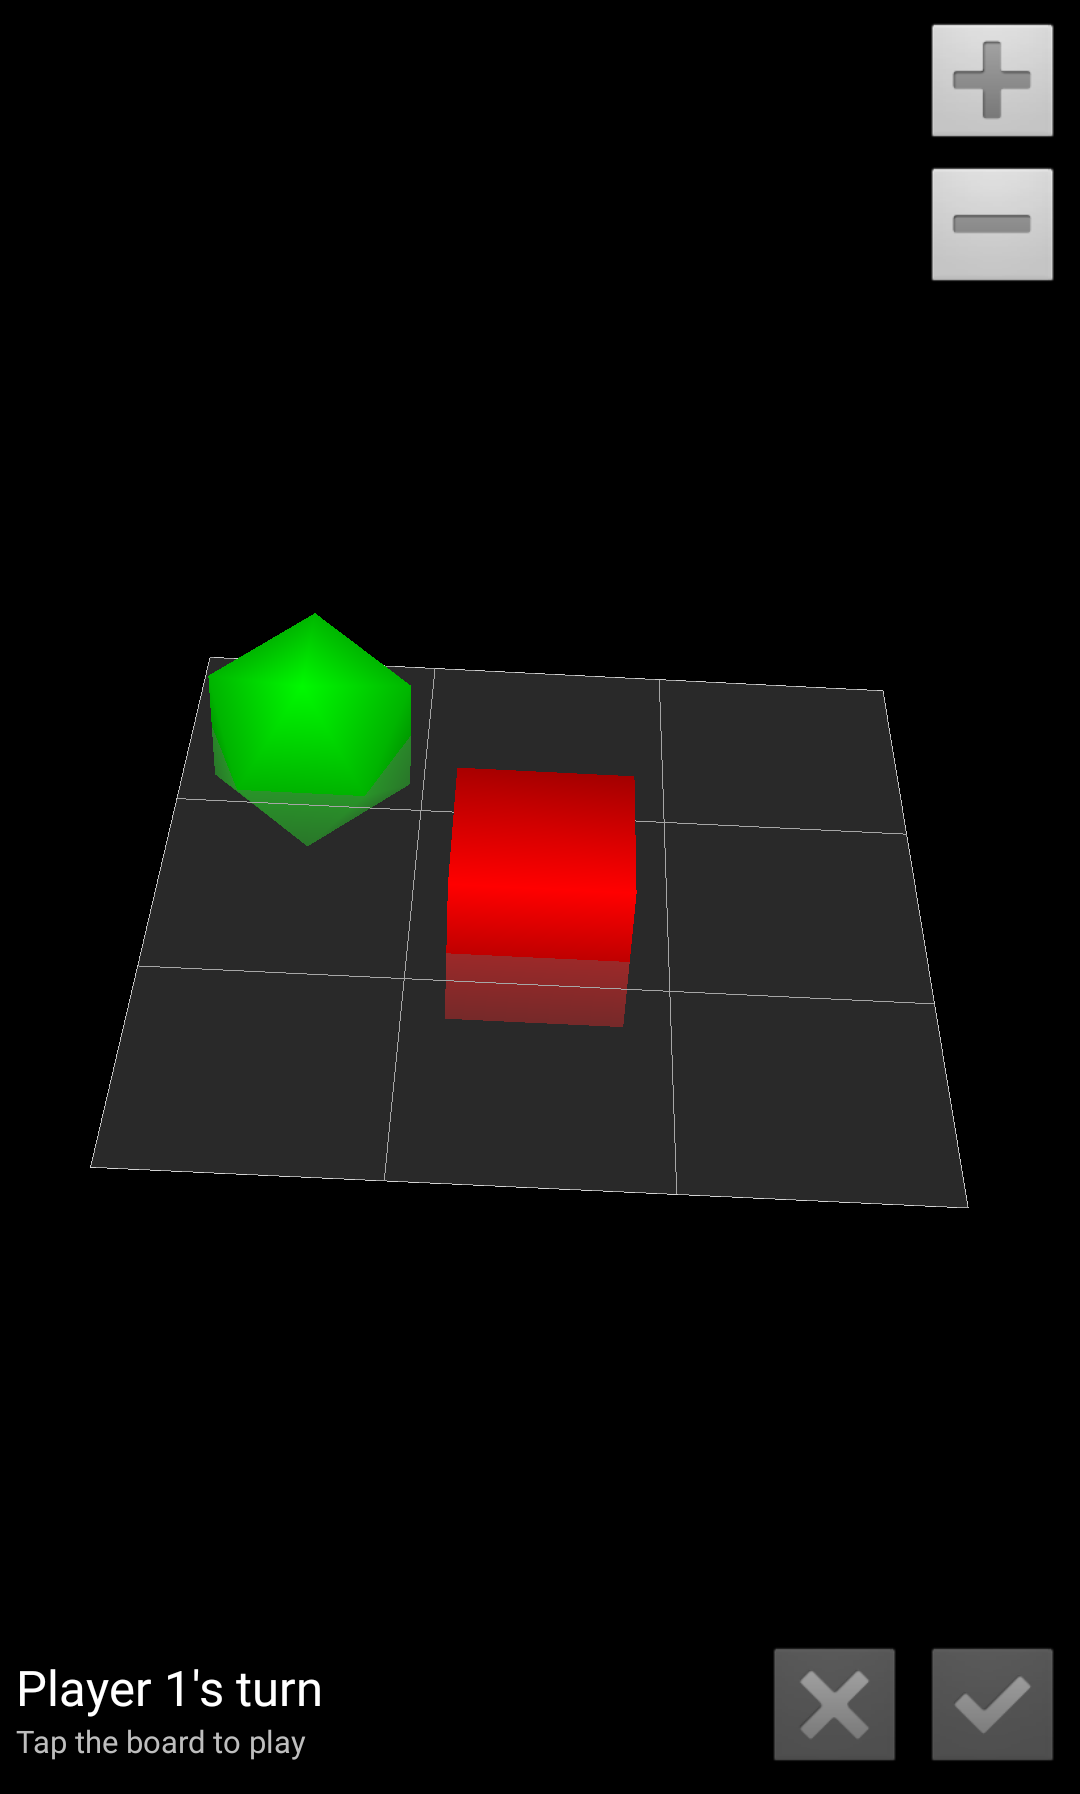
\includegraphics[height=11.1cm, keepaspectratio]{Analogs/AimlesscreativityGameplay.png}
    \caption{Игровой процесс игры Tic Tac Toe Pro (aimlesscreativity)}
    \label{Figure:Analysis:AimlesscreativityGameplay}
\end{figure}


\subsubsection{Крестики-нолики (VMSoft)}

Крестики-нолики 2 (VMSoft) -- одна из версий игры. Из достоинств можно отметить небольшие системные требования к устройству и высокое энергосбережение, также присутствует возможность как многопользовательской игры по сети интернет, так и игры против компьютерного противника \cite{VMSoft}.

К минусам приложения можно отнести следующее:
\begin{itemize}
    \item у игры отсутствует свой визуальный стиль и неудобное управление (рисунок \ref{Figure:Analysis:VMSoftGameplay}). По большему счёту это приложение, а не игра;
    \item отсутствует игровой режим с трёхмерным игровым полем;
    \item отсутствует версия под операционную систему iOS;
    \item для многопользовательской игры по сети интернет требуется наличие у пользователя сторонних сервисов.
\end{itemize}

\begin{figure}
\centering
    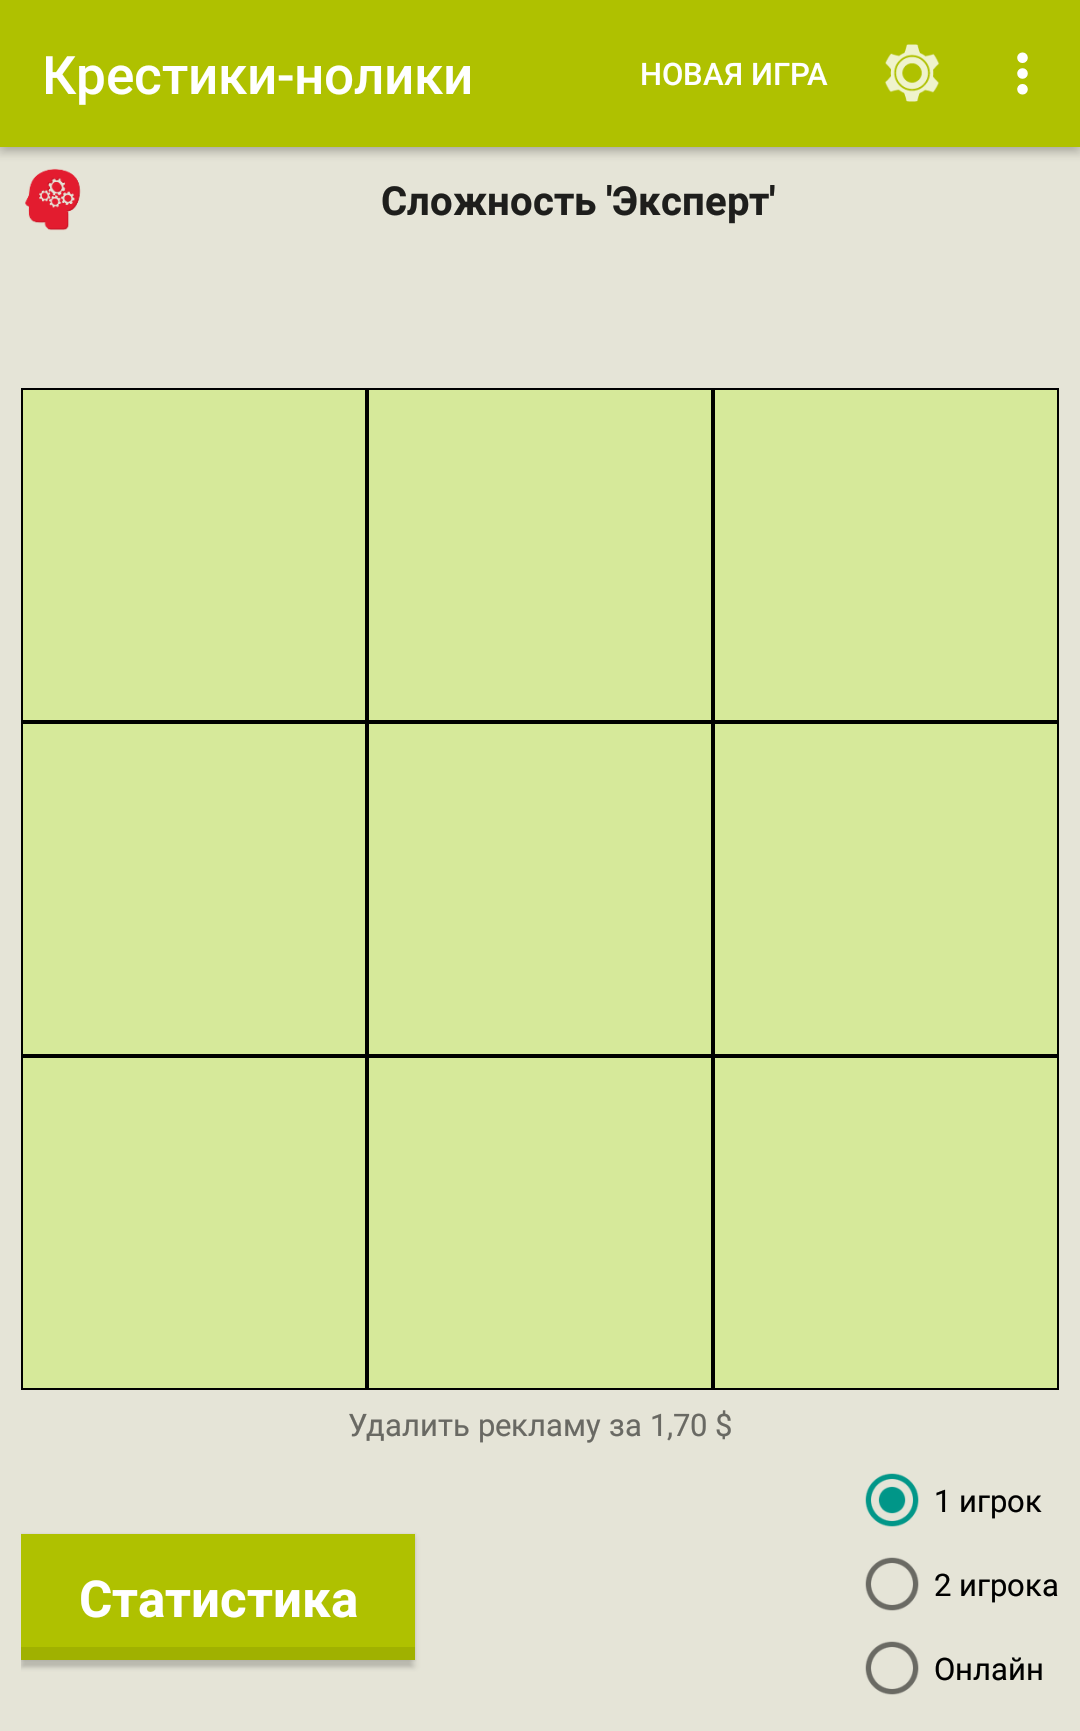
\includegraphics[height=11.1cm,keepaspectratio]{Analogs/VMSoftGameplay.png}
    \caption{Игровой процесс игры Крестики-нолики (VMSoft)}
    \label{Figure:Analysis:VMSoftGameplay}
\end{figure}


\subsubsection{Tic Tac Toe Glow (Arclite Systems)}

Tic Tac Toe Glow (Arclite Systems) -- неплохая версия игры, обладающая самым большим количеством скачиваний среди других версий на операционной системе Android. Игра обладает своим визуальным стилем (рисунки \ref{Figure:Analysis:ArcliteMainMenu} и \ref{Figure:Analysis:ArcliteGameplay}), присутствует возможностью играть по сети или с компьютерным противником, при этом многопользовательская игра по сети интернет не требует наличия у пользователя сторонних сервисов \cite{ArcliteSystems}.

К минусам приложения можно отнести следующее:
\begin{itemize}
    \item отсутствует игровой режим с трёхмерным игровым полем;
    \item отсутствует версия под операционную систему iOS.
\end{itemize}

\begin{figure}
    \centering
    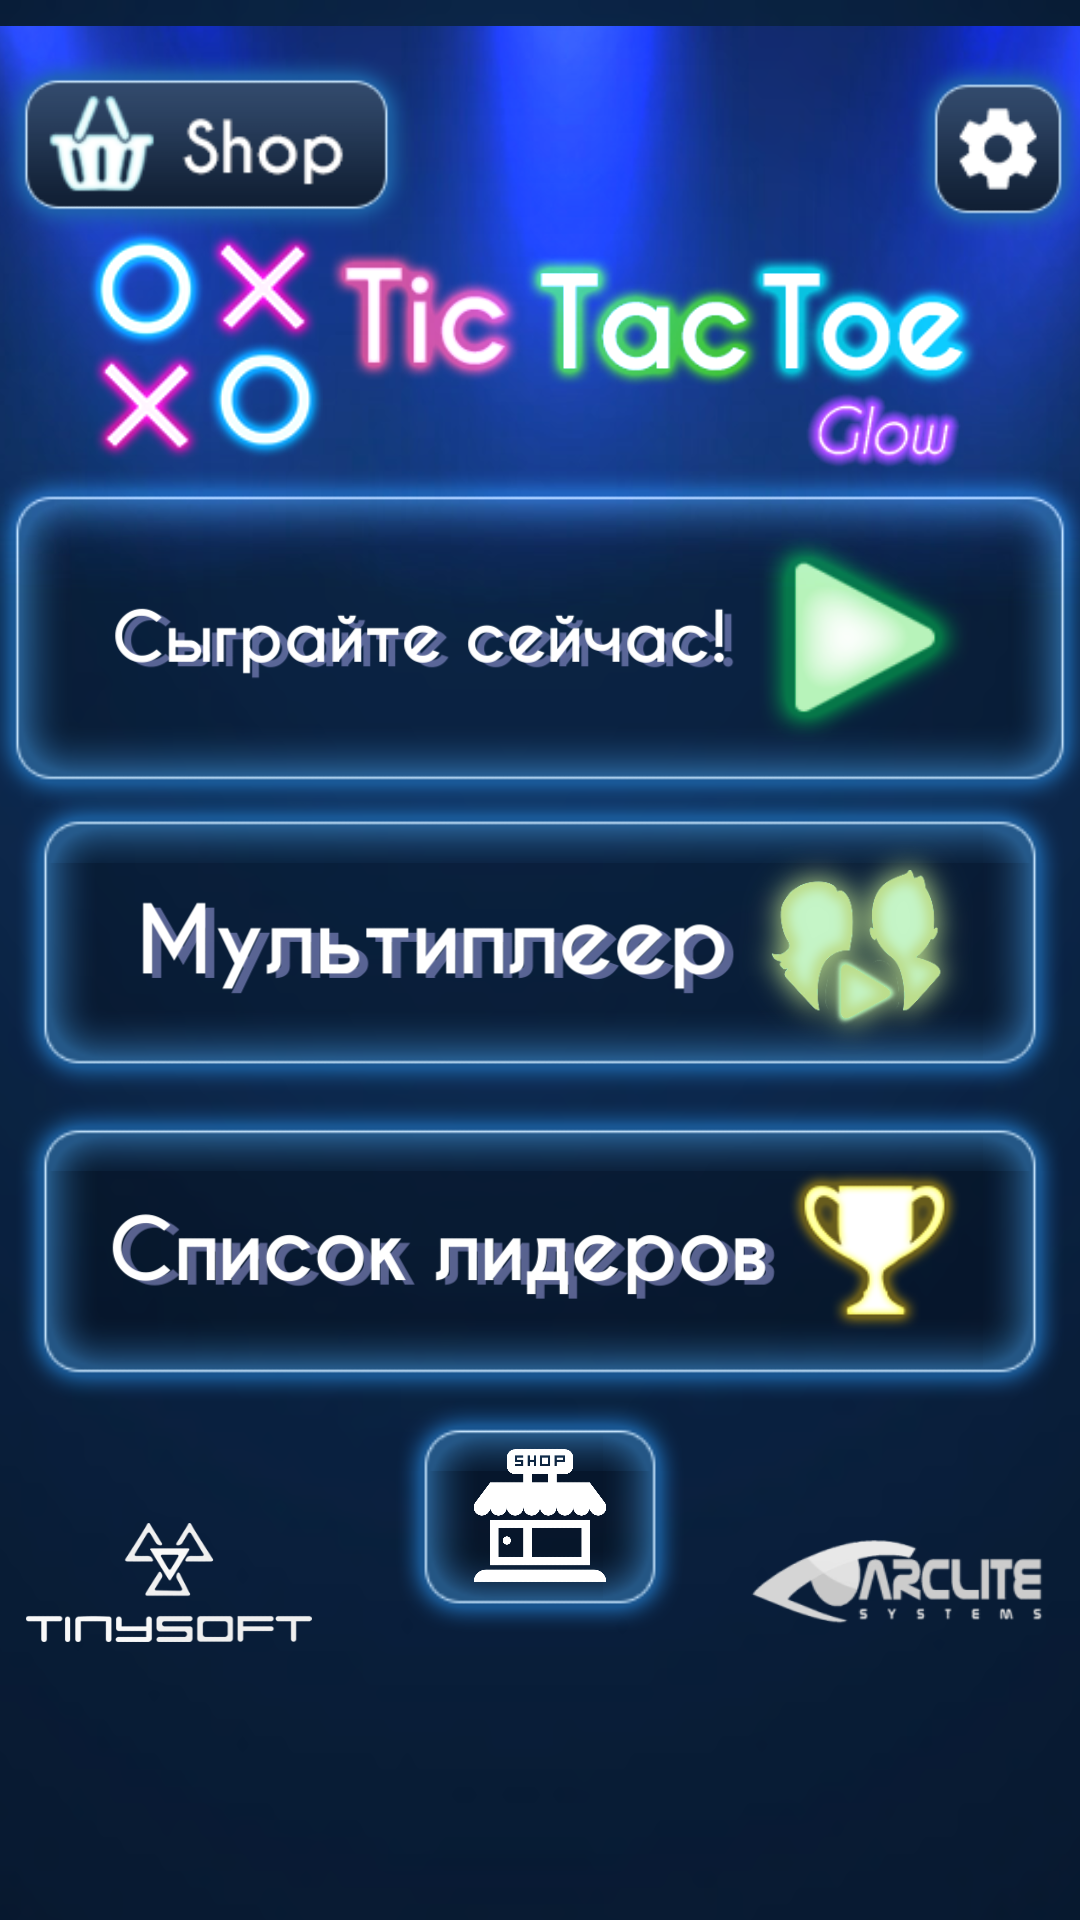
\includegraphics[height=11.1cm, keepaspectratio]{Analogs/ArcliteMainMenu.png}
    \caption{Главное меню игры Tic Tac Toe Glow (Arclite Systems)}
    \label{Figure:Analysis:ArcliteMainMenu}
\end{figure}

\begin{figure}
    \centering
    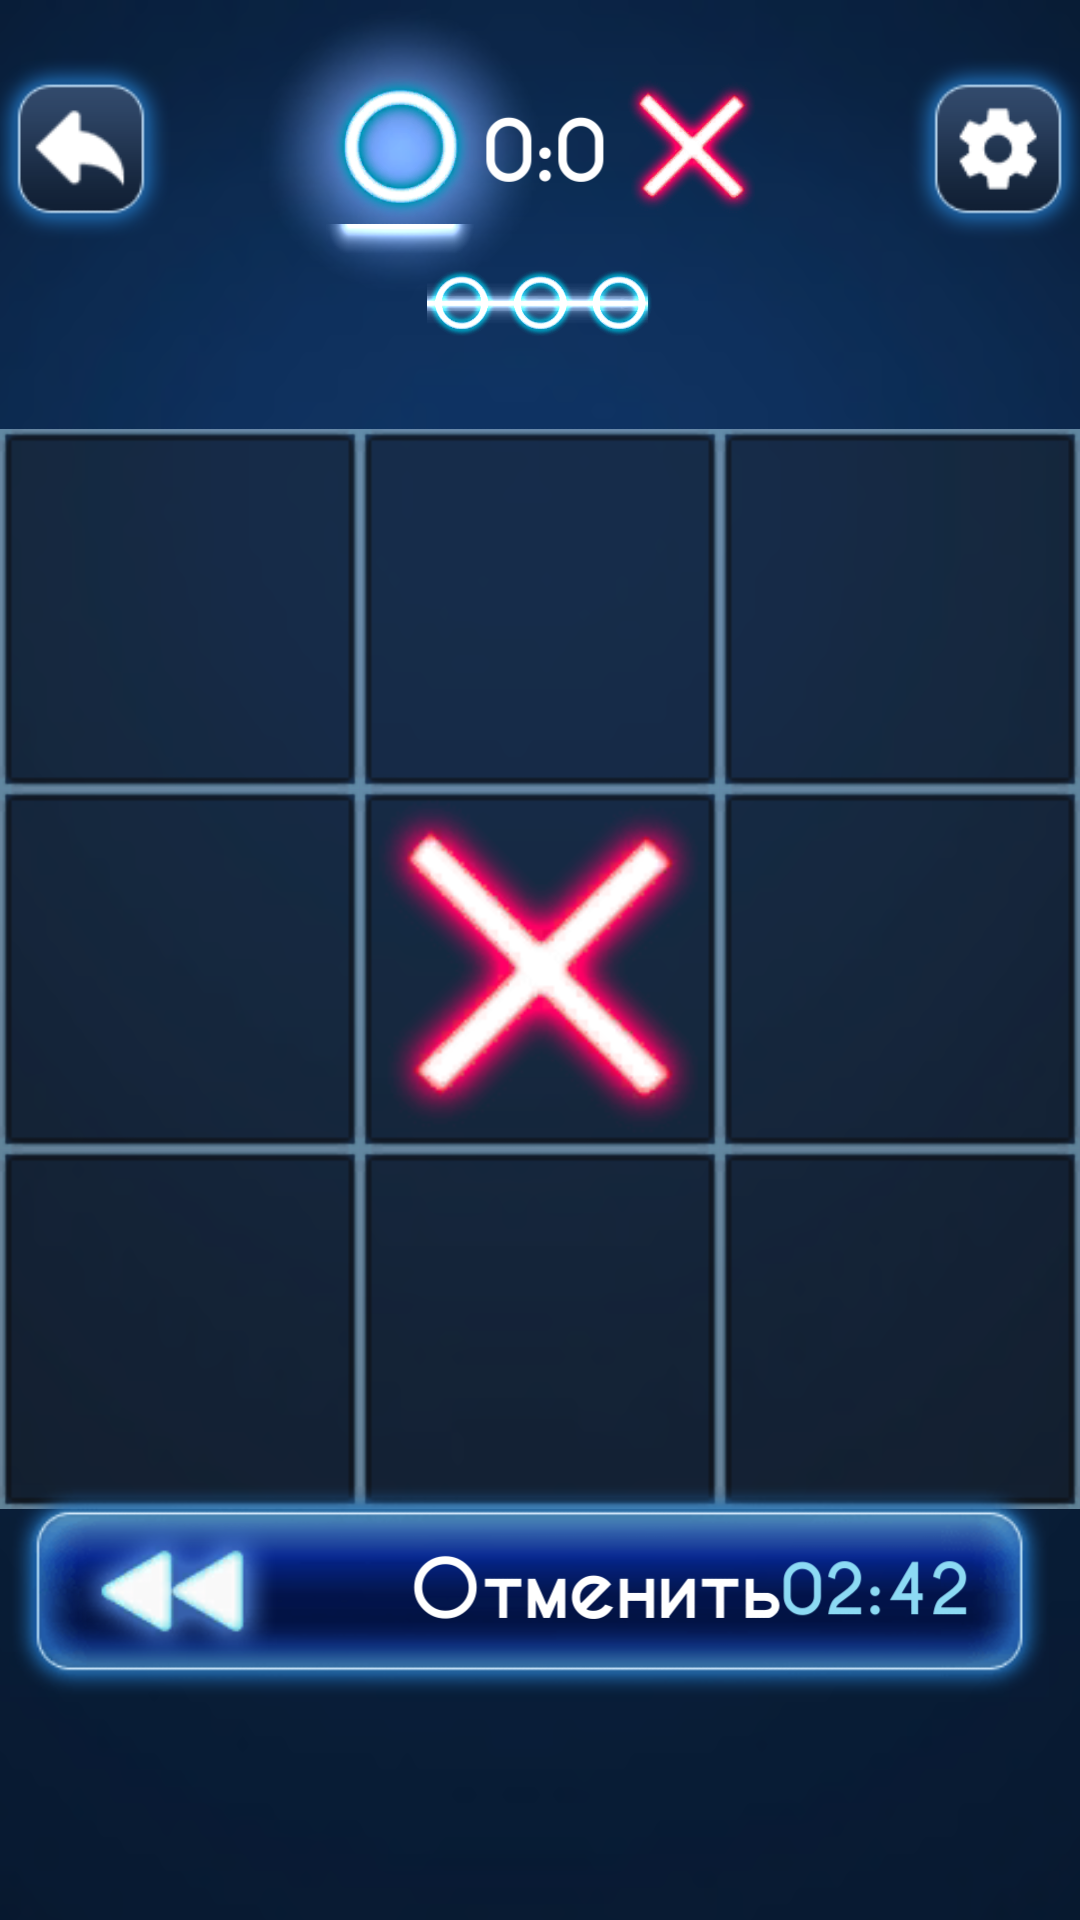
\includegraphics[height=11.1cm, keepaspectratio]{Analogs/ArcliteGameplay.png}
    \caption{Игровой процесс игры Tic Tac Toe Glow (Arclite Systems)}
    \label{Figure:Analysis:ArcliteGameplay}
\end{figure}


\subsubsection{Резюме}

Выше были рассмотрены четыре аналога создаваемого программного продукта. Каждый из них обладает как плюсами, так и минусами, но стоит выделить тот факт, что все они имеют версию только для одной целевой операционной системы и в большинстве из них для многопользовательской игры требуется наличие у пользователя сторонних сервисов.